\section{Definizioni e Esposizione dei concetti}
\subsection{Algoritmo}
Per definizione un algoritmo è una sequenza finita di passi base, o operazioni, utili a risolvere un problema, in genere matematico. Essi sono di fondamentale importanza in quanto possono essere la formalizzazione di operazioni svolte da un computer e l'informatica (almeno nella sua parte più scientifica) è la disciplina che li tratta. Storicamente i passi base sono diventati sempre più astratti: se inizialmente trattavano della gestione della memoria byte per byte e di operazioni come porte logiche ad oggi il linguaggio è sempre più matematico e discorsivo non esplicitando quello che avviene a livello hardware. Essendo i computer e la computazione quantistica una tecnologia a livello ancora "embrionale" e di fatto molto più complessa del corrispettivo classico un linguaggio astratto non è ancora sviluppato.
\subsection{Complessità}
La complessità è una proprietà di ogni algoritmo ed indica quanto veloce o lento esso viene eseguito (si parla di complessità temporale) oppure quanta memoria deve occupare (si parla di complessità di memoria).
In genere la memoria è di secondaria importanza in quanto i calcolatori attuali (soprattutto se si prendono in considerazione i supercomputer) ne dispongono di sufficiente per la maggior parte dei problemi, ma la complessità temporale è fondamentale in quanto un particolare problema è necessario che sia risolto oggi e non tra qualche anno o addirittura nemmeno domani.\\
Essa viene espressa da una funzione \textit{T(N)} tempo su dimensione dei dati in input. Dovendo un algoritmo risolvere non solo un'istanza di un problema, ma tutti i casi possibili chiaramente il tempo impiegato dipende anche dai dati di partenza; in particolar modo dalla loro quantità e dimensione (cioè quanta memoria occupano). Essendo ogni calcolatore diverso e diventando più potenti con l'avanzare del tempo \textit{T(N)} non viene espresso in secondi dato che sarebbe diverso per ogni hardware, ma in numero di passi base che dipende solo dall'algoritmo in sè. Anche questo metodo è però troppo specifico in quanto esprimere \textit{T(N)} può essere molto difficile oppure pieno di dati poco importanti; viene quindi usata la notazione \textit{O-grande} cioè una funzione \textit{O(f(N))} che esprime l'andamento della complessità, più precisamente:
$T(N) := O(f(N)) \iff \exists \ C\times f(N) > T(N)\ \forall \ N \geq n0 \ | \ C,n0 \in \ \mathbb{R} $\\
Cioè un algoritmo si può dire \textit{O(f(N))} se e solo se f(n) moltiplicato per una certa costante è sempre maggiore di \textit{T(N)} da un certo punto in poi. Questa notazione è ottima in quanto dove non funziona (cioè per N molto piccoli) il tempo impiegato è talmente poco che non ci si può accorgere dell'errore e dove funziona (per N grandi) esprime con semplicità e ottima approssimazione il tempo impiegato (eliminando fattori di poca importanza).\\
Tutti i problemi del mondo vengono classificati in relazione alla complessità migliore ottenibile dagli algoritmi risolventi; una prima distinzione viene fatta tra i problemi non calcolabili e quelli calcolabili, cioè quelli per cui non può e può esistere un algoritmo risolvente. Poi ognuno dei calcolabili appartiene all'insieme \textbf{NP} (Non Polinomiale) in cui può esistere un algoritmo in grado di risolvere i problemi con una complessità non polinomiale (cioè in \textit{O(f(N))} f(N) non è polinomiale) e un sottoinsieme di essi appartiene anche a \textbf{P} (Polinomiale) ove può esistere un algoritmo in grado di risolverli in tempo polinomiale. Da porre attenzione però al fatto che polinomiale e non polinomiale in questo caso non hanno il vero significato matematico in quanto all'insieme dei polinomiali appartengono anche alcune funzioni come le logaritmiche; per NP si intende più che altro funzioni che crescono più velocemente delle polinomiali.\\
All'interno di P si distinguono poi numerosissime classi a seconda delle  varie f(N), di seguito un elenco delle più famose (in ordine dalla più veloce):\\
\textit{O(1)}, \textit{O(logN)}, \textit{O($\sqrt{N}$)}, \textit{O(N)}, \textit{O(NlogN)}, \textit{O($N^2$)}, \textit{O($N^k$)}...
\section{Esempi classici}
Alcuni esempi di algoritmi classici. La somma con le porte logiche, la ricerca lineare e la ricerca binaria.
\subsection{Somma}
Sommare due numeri è relativamente semplice per il cervello umano, ma non immediato per una macchina; ricordiamo infatti che le uniche operazioni che può fare in modo diretto tra bit sono date dalle porte logiche e quindi bisogna trovare un modo di combinarle per fare in modo che a partire da due bit si ottenga la somma.\\
Per capire meglio partiamo dall'esempio di voler sommare 6 e 7, a mente il risultato è immediato, ma basiamoci sulla struttura delle somme in colonna:
\begin{lstlisting}[language=python]
   6
+  7
----
= 13
\end{lstlisting}
Il ragionamento è che 6+7 vale 3 con il resto di 1 che va portato alla colonna successiva in cui non c'è nulla e quindi alla fine 13.\\
I numeri sono però in formato binario nei computer, ma non è un problema in quanto la regola vale comunque, è anzi più semplice in quanto ci sono solo due possibili cifre; 6 è 110, mentre 7 111:
\begin{lstlisting}[language=python]
   110
+  111
------
= 1101
\end{lstlisting}
Il ragionamento è che 1+0 sia 1 senza resto, poi 1+1 sia 0 con il resto di 1 e infine 1+1+1 è 1 con il resto di uno che rimane su una colonna vuota; quindi il risultato è 1101, il corrispondente di 13.\\
Partendo da analizzare una sola colonna si ha bisogno di un circuito che dati due bit di partenza dia come risultato 1 se solo uno dei due vale 1 (e quindi una porta \textit{XOR}), 0 altrimenti e come resto 1 solo se entrambi valgono 1 (quindi una porta \textit{AND}). Nell'immagine qui sotto A e B sono gli input mentre S il risultato e C il resto. Il rettangolo con la scritta "Half Adder" è il riassunto del circuito sopra con a sinistra gli input e a destra gli output.
\begin{center}
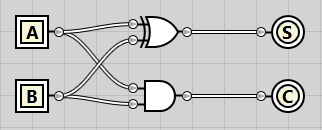
\includegraphics[scale=1.3]{halfSum}\\
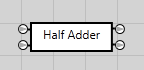
\includegraphics[scale=1]{halfSumIco}
\end{center}
Questo circuito però non basta a sommare una colonna qualsiasi in quanto potrebbe esserci il resto dalla colonna prima, è quindi necessario un circuito piò complicato, chiamato "Full Adder". I quadrati A (primo bit), B (secondo bit) e C (resto precedente) sono gli input, i cerchi S e C gli output.
\begin{center}
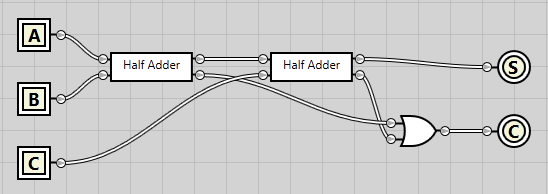
\includegraphics[scale=0.9]{fullAdder}
\end{center}
Ora che è possibile sommare una colonna per sommarne di più basta concatenare i "Full Adder" in modo  che il resto ogni volta faccia parte della colonna successiva; ad oggi i processori sono disegnati per maneggiare fino a 64 bit per volta, ma nell'immagine qui sotto un esempio di 3, in cui si svolge 7+3 (il rosso corrisponde a 1, il bianco a 0):
\begin{center}
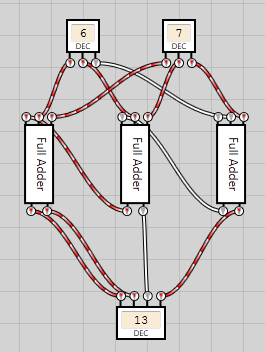
\includegraphics[scale=0.9]{triAdder}
\end{center}
\subsection{Ricerca lineare}
Data una lista casuale di elementi determinare se un preciso elemento denominato X esiste e in che posizione si trova.\\
Questo problema viene risolto da un algoritmo di ricerca molto semplice: controllare ogni elemento partendo dal primo e verificare se esso è uguale ad X; in pseudo-codice:
\begin{lstlisting}[language=python]
posizione = None
contatore = 1
for elemento in lista:
	if elemento = X:
		posizione <- contatore
	contatore = contatore + 1
return posizione
\end{lstlisting}
Dovendo potenzialmente analizzare tutta la lista la complessità di questo algoritmo è \textit{O(N)}
\subsection{Ricerca binaria}
Il problema cui si vuole trovare soluzione è lo stesso dell'esempio precedente, ma la lista, invece che essere casuale, è ordinata. Certamente la ricerca lineare funzionerebbe comunque, ma nello specifico caso è possibile usare una variante più efficiente.\\
Invece di iniziare dal primo elemento si parte da quello centrale e si verifica se si trova prima o dopo dell'elemento cercato (se sono numeri ad esempio si controlla se è maggiore o minore) e si restringono gli estremi della lista di conseguenza; se ad esempio l'elemento si trova primo di quello centrale si può eliminare dalla ricerca la seconda metà della lista. Lo stesso procedimento si applica a ripetizione continuando ad accorciare la lista di interesse. In questo modo è anche possibile trovare la posizione che occuperebbe l'elemento in caso non sia presente oppure gli elementi più simili. Nell'esempio qui sotto viene trovata la posizione dell'elemento minore o uguale ad X:
\begin{lstlisting}[language=python]
inizio = 1
fine = length(lista)
while inizio < fine:
	mezzo = (inizio + fine)/2
	if lista[mezzo] < X:
		fine = mezzo
	else:
		inizio = mezzo
return mezzo
\end{lstlisting}
Si può facilmente dimostrare come con questo algoritmo si venga a creare un albero binario di scelte (difatti ad ogni iterazione si scegle se prendere il sottoinsieme di destra o sinistra) che ha come base gli elementi singoli della lista. Per trovarne uno è necessario percorre tutto un ramo (e quindi l'altezza dell'albero) che è lungo \textit{$\log_22$} volte la base; la complessità è quindi \textit{O(log(N))}
\subsection{Commesso viaggiatore}
Il problema è: Viene data una lista di città e la descrizione delle strade che le collegano; in particolare quali sono e quanto tempo impiegano ad essere percorse. Si vuole trovare il percorso che partendo da una determinata città le attreversi tutte e ritorni impiegando meno tempo possibile.\\
L'unico modo per risolverlo è provare ogni singolo percorso, e, dato che il numero delle combinazioni cresce in modo esponenziale con l'aggiunta di città e strade, il problema rientra nella classe NP. Questo significa che oltre un certo (abbastanza basso) numero di città il tempo che si impiega per calcolare il percorso migliore può essere di anni o anche millenni il che rende (se non nella teoria) nella pratica impossibile risolvere il problema.
\section{Esempi quantistici}
Le macchine quantistiche hanno la possibilità di sfruttare ogni algoritmo classico (ma non conviene in quanto sono molto più costose e difficili da costruire), però non è vero il contrario; esistono algoritmi che possono essere eseguiti solo da computer quantistici.
Questi ultimi in genere risolvono alcuni problemi calcolabili con una complessità minore degli algoritmi classici; in particolare un sottoinsieme dei Non Polinomiali (chiamato EQP) se approcciato con una macchina quantistica rientra nei Polinomiali. (Questo ovviamente non funziona per tutti i problemi, ad esempio il commesso viaggiatore rimane NP).\\
Essendo la maggior parte di questi algoritmi molto complessi sia dal punto di vista informatico che matematico (richiedendo conoscenza approfondita di algebra lineare) gli algoritmi non verranno approfonditi, ma solo esposti.
\subsection{Deutsch-Josza}
Disponiamo di una scatola nera che implementa una funzione \textit{$f: \{0,1\}^n \rightarrow \{0,1\}$} cioè prende in input \textit{n} bit e ha un output di uno solo. Di questa funzione si sa solo che può essere o costante (cioè per tutti gli input restituisce un solo risultato) oppure bilanciata (e quindi per esattamente metà restituisce 1 e per l'altra metà 0). Viene richiesto quindi di determinare se \textit{f} è costante o bilanciata.
Questo è il problema che l'algoritmo di Deutsch-Josza deve risolvere.
\subsubsection{Approccio classico}
Innanzitutto si può notare che esso è risolvibile anche in modo classico: si possono provare in ordine varie combinazioni degli \textit{n} bit e verificare come si comporta \textit{f}. Nel caso ottimo bastano due test, se il risultato è diverso sicuramente la funzione non può essere costante e quindi è bilanciata; nel caso pessimo però è necessario provare almeno la metà più uno in quanto finchè otteniamo risultati identici non possiamo essere sicuri che \textit{f} sia costante finchè essi non sono più della metà. La complessità di un approccio classico è infatti \textit{O($2^n$)} in quanto, essendo $2^n$ le possibili combinazioni, ne vanno testate in media $2^{n-1} + 1$.
\subsubsection{Approccio quantistico}
Nel caso in cui la scatola nera sia una macchina quantistica e quindi non rompa la superposizione dell'input è possibile applicare l'algoritmo (quantistico) di Deutsch-Josza. Il concetto è che invece di dare in input una combinazione precisa, ogni singolo qubit è in sovrapposizione con egual probabilità di essere 0 o 1. Si ottiene quindi una correlazione tra input e output la quale ha probabilità di avere valore 0 nulla solo se \textit{f(x)} è bilanciato e valore 1 se \textit{f(x)} è costante (per interferenza distruttiva e costruttiva).
Per più informazioni a riguardo:\\
$\href{https://bit.ly/2MwuZRI}{bit.ly/2MwuZRI}$\\
La complessità di questo algoritmo è \textit{O(N)} in quanto richiede solo di preparare una combinazione, il che è un'accelerazione esponenziale rispetto all'algoritmo classico.
\subsection{Grover}
Per l'algoritmo di Grover il problema è la ricerca in una lista casuale (come la ricerca lineare) con un approccio quantistico.\\
Nell'algoritmo viene costruita una sovrapposizione di qubit in modo tale che ogni indice sia equiprobabile, vengono poi applicate delle trasformazioni al sistema in modo tale che la probabilità dell'indice corretto aumenti; questo viene ripetuto un numero tale di volte da massimizzare la probabilità che il sistema collassi all'indice corretto, si può dimostrare che il numero è dell'ordine di $\sqrt{N}$.
La probabilità di ottenerlo però non arriva mai a 1 e quindi si può ottenere un risultato sbagliato; per questo l'algoritmo non è deterministico, ma dato che essa non dipende da N ripetere l'esecuzione dell'algoritmo solo poche volte rende la probabilità di errore molto prossima allo  0. La complessità dell'algoritmo è quindi \textit{O($\sqrt{N}$)}.
Per approfondimenti:\\
$\href{https://bit.ly/1ubOwWj}{bit.ly/1ubOwWj}$
\subsection{Shor}
Il problema che viene affrontato dall'algoritmo di Shor a parole è relativamente semplice: Fattorizzare un numero. Vediamo innanzitutto come risolverlo da un punto di vista classico.
\subsubsection{Approccio classico}
Non esistendo alcuno stratagemma veloce per determinare quali primi dividono un numero qualsiasi è necessario provare tutti quelli minori del numero da dividere. Sfortunatamente però non esiste nemmeno un modo istantaneo per discernere un numero primo da un non primo e nemmeno uno che ci permette di capire quale sia il numero primo successivo a uno dato; quindi non solo bisogna tentare tutti i primi minori del numero, ma bensì tutti (o quasi) i numeri minori; se ad esempio volessimo scomporre 308 il procedimento sarebbe il seguente:
Si tenta di dividere per 2 308, è possibile quindi 2 è un fattore, otteniamo 154. Si riprova con 2 ed è dividibile, otteniamo 77. Esso non è divisibile per 2, nè per 3, nè per 5, ma invece per 7 sì (si possono saltare i fattori pari) otteniamo 11. Esso non è divisibile per 7, nemmeno per 9 ma per 11; otteniamo 1. Essendo 11 maggiore di 1 possiamo fermarci.\\
308 viene quindi scomposto in $2^2 \times 7 \times 11$. Si può notare come potenzialmente ci si può spingere fino a $\sqrt{M}$ (dove M è il numero) e l'insieme dei numeri compresi tra 2 e $\sqrt{M}$ cresce in modo esponenziale rispetto al numero di cifre (chiamato N) di M, perciò aggiungere una cifra al numero da scomporre rende l'algoritmo esponenzialmente più lento. La complessità si può quindi denotare approssimativamente con \textit{O($2^N$)}.
\subsubsection{Approccio quantistico}
La chiave dell'algoritmo quantistico di Shor sta nel processo di ricerca del periodo di una funzione svolto dalla \textit{trasformata di Fourier quantistica} (\textbf{QFT}). Per capire come essa funzioni riporto l'analogia del professor Scott Aarson tradotta in italiano:
\begin{displayquote}
Immaginiamo che io abbia degli orari molto strani; in particolare la mia giornata dura più di 24 ore. Se ti dicessi che oggi mi sono svegliato alle 5 del pomeriggio sapresti dirmi quanto di preciso dura: 25, 26, 27.4...? Certo che no, infatti in ogni caso la mia sveglia cambierebbe ogni giorno e prima o poi nella maggior parte dei casi capiterà che arrivi alle 5 del pomeriggio.\\
Ora immaginiamo che il muro della mia camera sia pieno di orologi analogici, ma tutti diversi: in ognuno di essi la lancetta delle ore per compiere un giro intero ci impiega un tempo diverso e per di più esiste un orologio per ogni periodo cui si possa pensare. Poi sotto ognuno è presente un poster cui è attaccata una puntina. Ti posso assicurare che la prima volta che ho dormito nell'appartamento ho posizionato le puntine al centro di ogni poster, poi però ogni giorno subito dopo essermi svegliato spostavo le puntine di un centimetro nella direzione indicata dalla lancetta.\\
Ora, esaminando le puntine, si può affermare con sicurezza la durata della mia giornata? Assicuro che sì, è possibile. Per esempio se la mia giornata fossse di 26 ore si può dedurre che il moto della puntina sotto l'orologio delle 24 ore sia periodico; ogni giorno la lancetta punta in posizioni diverse e prima o poi ritornerà nella posizione iniziale.\\
Cosa accade però alla puntina sotto l'orologio delle 26 ore? Essendo in sincrono con la mia giornata ogni volta che mi sveglio la lancetta punta sempre la stessa ora, e quindi la stessa direzione, perciò la puntina si muoverà sempre nella stessa direzione. L'importante è che questo accade solo per l'orologio delle 26 ore.
\begin{center}
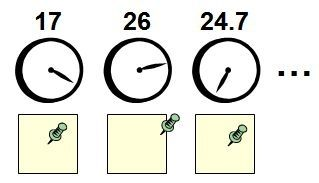
\includegraphics[scale=1]{ShorClocks}
\end{center}
Infine quindi per determinare la durata della mia giornata basta solo cercare l'orologio la cui puntina è più lontana dal punto iniziale.
\end{displayquote}
Questo è quello che accade nel QFT: una serie di qubit in sovrapposizione rappresentano contemporaneamente tutti i possibili periodi, poi per interferenza costruttiva quello corretto diviene sempre più probabile a discapito degli altri, così che quando il sistema collassa molto probabilmente sarà sul periodo corretto.\\
Successivamente ci si può avvalere della matematica classica difatti per fattorizzare un numero \textit{N} basterà scegliere un numero casuale minore di N chiamato \textit{a} e cercare la periodicità di $a^x mod N$ (Dove \textit{mod} rappresenta il resto della divisione. A questo punto è dimostrabile come il Massimo Comun Divisore di $a^\frac{periodo}{2}$-1 e N è un fattore di N e quindi la soluzione.\\
Questo non funziona per tutti gli \textit{a}, ma è molto più probabile un esito positivo piuttosto che negativo; quindi è sufficiente provarne pochi.
Calcolare la complessità non è semplice, in quanto dipende da come l'algoritmo viene implementato, ma dovrebbe essere intorno a \textit{O($N^3$)} il che è un'accelerazione esponenziale rispetto all'algoritmo classico.
Per approfondire:\\
\href{https://bit.ly/2tfo86l}{bit.ly/2tfo86l}